\section{SM and beyond: Allowed, forbidden and discovery process}
\begin{enumerate}
  \item
    \begin{enumerate}
      \item
	\begin{itemize}
      	  \item Electromagnetic
      	    \begin{itemize}
      	      \item 1, 2, 3, 4, 6, 8, 11, 12, 13, 14, 15, 16, 20
      	    \end{itemize}
      	  \item Weak
      	    \begin{itemize}
      	      \item 5, 7, 10, 13, 18, 19
      	    \end{itemize}
      	\end{itemize}
      \item
	Particle decay, lifetime and branching
      \item
	Conservation laws, suppression, etc.
      \item
	process 3,4,8,10,11, 14 and 18 more important
    \end{enumerate}
\end{enumerate}
\newgeometry{left=0.5cm,right=0.5cm,top=0.2cm,bottom=1.3cm}
\begin{figure}[h]
  \centering
  \begin{subfigure}[b]{0.3\textwidth}
    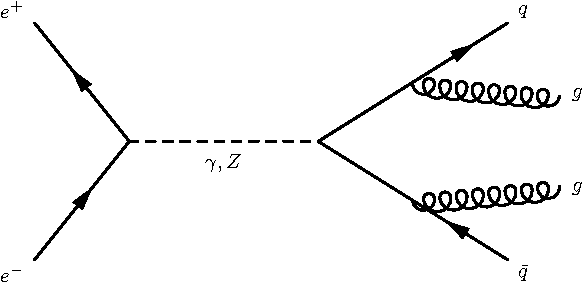
\includegraphics[width=\textwidth]{../dia/01.pdf}
    \caption{$e^+e^- \rightarrow q\bar{q}gg$}
    \label{fey:1}
  \end{subfigure}%
  ~
  \begin{subfigure}[b]{0.3\textwidth}
    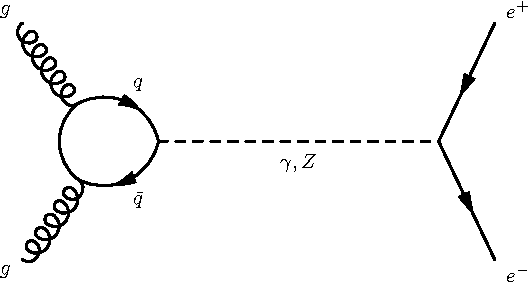
\includegraphics[width=\textwidth]{../dia/02.pdf}
    \caption{$gg\rightarrow e^+e^-$}
    \label{fey:2}
  \end{subfigure}%
  ~
  \begin{subfigure}[b]{0.3\textwidth}
    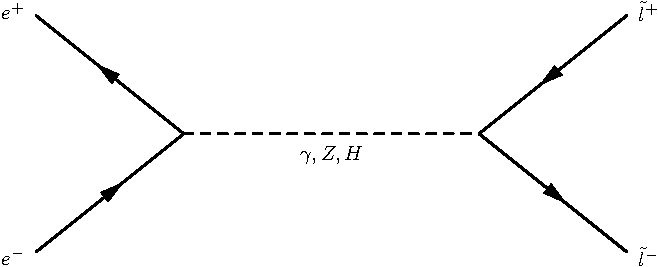
\includegraphics[width=\textwidth]{../dia/03.pdf}
    \caption{$e^+e^-\rightarrow \tilde{l}^+\tilde{l}^-$}
    \label{fey:3}
  \end{subfigure}
  \newline
  \newline
  \begin{subfigure}[b]{0.3\textwidth}
    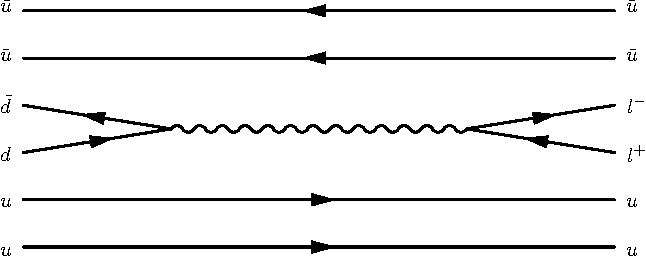
\includegraphics[width=\textwidth]{../dia/04.pdf}
    \caption{$p\bar{p}\rightarrow l^+l^-x$}
    \label{fey:4}
  \end{subfigure}%
  ~
  \begin{subfigure}[b]{0.3\textwidth}
    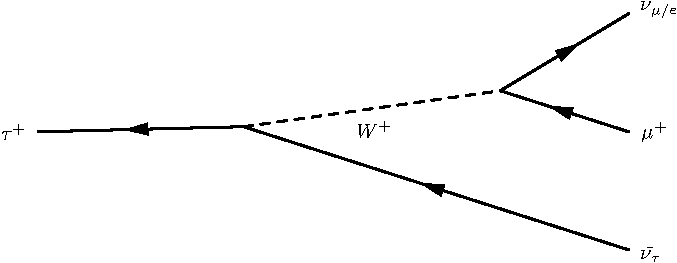
\includegraphics[width=\textwidth]{../dia/05.pdf}
    \caption{$\tau^+\rightarrow \mu^+\bar{\nu}_{\tau}\nu_{e/\mu}$}
    \label{fey:5}
  \end{subfigure}%
  ~
  \begin{subfigure}[b]{0.3\textwidth}
    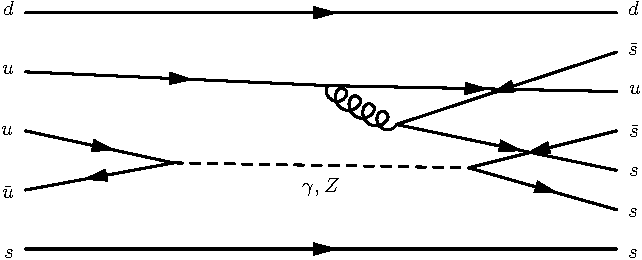
\includegraphics[width=\textwidth]{../dia/06.pdf}
    \caption{$k^-p\rightarrow \omega^-k^+k^0$}
    \label{fey:6}
  \end{subfigure}
  \newline
  \newline
  \begin{subfigure}[b]{0.3\textwidth}
    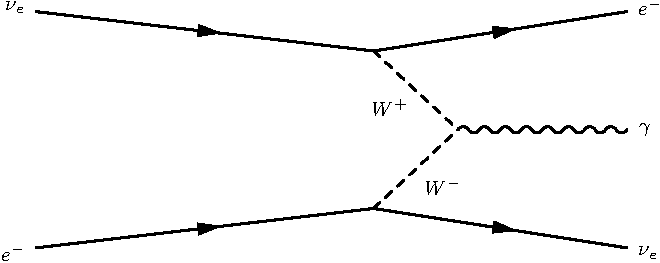
\includegraphics[width=\textwidth]{../dia/07.pdf}
    \caption{$e^-\nu_e\rightarrow \nu_e \gamma e^-$}
    \label{fey:7}
  \end{subfigure}%
  ~
  \begin{subfigure}[b]{0.3\textwidth}
    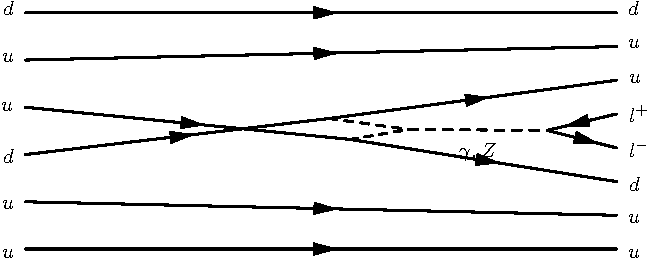
\includegraphics[width=\textwidth]{../dia/08.pdf}
    \caption{$pp\rightarrow ppl^+l^-$}
    \label{fey:8}
  \end{subfigure}%
  ~
  \begin{subfigure}[b]{0.3\textwidth}
    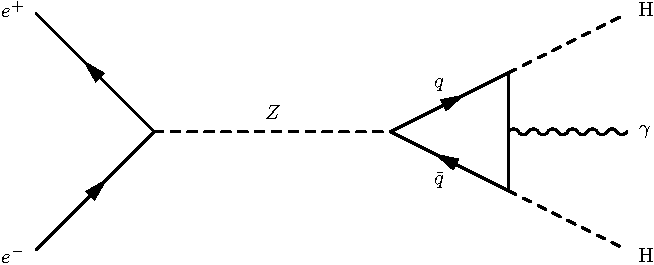
\includegraphics[width=\textwidth]{../dia/09.pdf}
    \caption{$e^-e^+ \rightarrow \gamma HH$}
    \label{fey:9}
  \end{subfigure}
  \newline
  \newline
  \begin{subfigure}[b]{0.3\textwidth}
    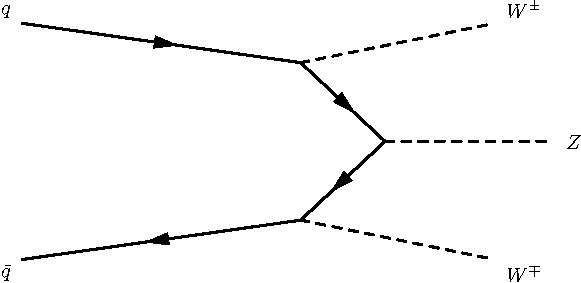
\includegraphics[width=\textwidth]{../dia/10.pdf}
    \caption{$qq\rightarrow W^{\pm}W^{\mp}Z$}
    \label{fey:10}
  \end{subfigure}%
  ~
  \begin{subfigure}[b]{0.3\textwidth}
    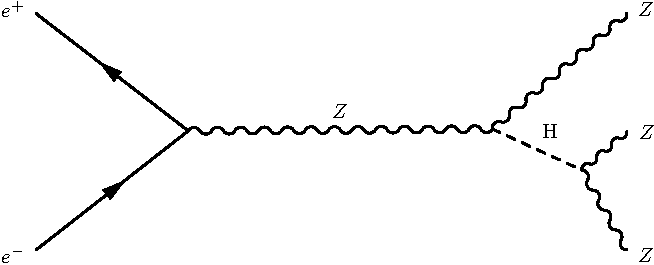
\includegraphics[width=\textwidth]{../dia/11.pdf}
    \caption{$e^-e^+\rightarrow ZZ$}
    \label{fey:11}
  \end{subfigure}%
  ~
  \begin{subfigure}[b]{0.3\textwidth}
    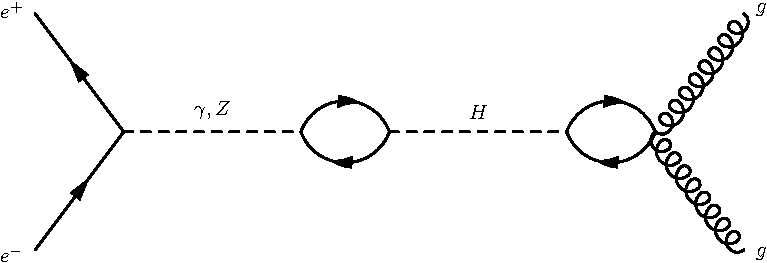
\includegraphics[width=\textwidth]{../dia/12.pdf}
    \caption{$e^-e^+\rightarrow H \rightarrow gg$}
    \label{fey:12}
  \end{subfigure}
  \newline
  \newline
  \begin{subfigure}[b]{0.3\textwidth}
    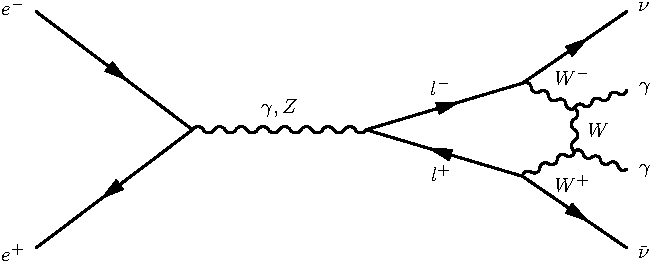
\includegraphics[width=\textwidth]{../dia/13.pdf}
    \caption{$e^+e^- \rightarrow \nu\bar{\nu}\gamma\gamma$}
    \label{fey:13}
  \end{subfigure}%
  ~
  \begin{subfigure}[b]{0.3\textwidth}
    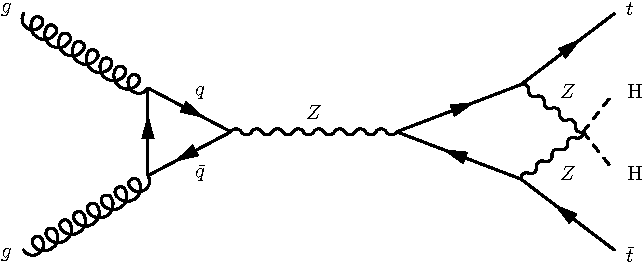
\includegraphics[width=\textwidth]{../dia/14.pdf}
    \caption{$gg\rightarrow t\bar{t}HH$}
    \label{fey:14}
  \end{subfigure}%
  ~
  \begin{subfigure}[b]{0.3\textwidth}
    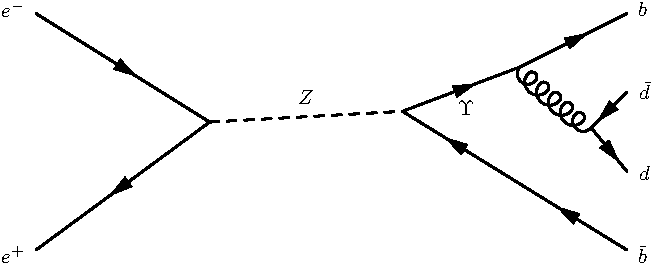
\includegraphics[width=\textwidth]{../dia/15.pdf}
    \caption{$e^+e^-\rightarrow \Upsilon(3s)\rightarrow B^0\bar{B^0}$}
    \label{fey:15}
  \end{subfigure}
  \newline
  \newline
  \begin{subfigure}[b]{0.3\textwidth}
    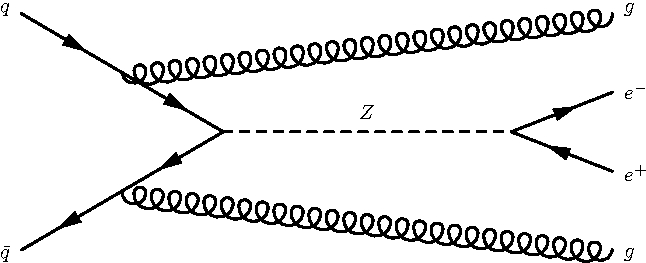
\includegraphics[width=\textwidth]{../dia/16.pdf}
    \caption{$q\bar{q}\rightarrow gge^-e^+$}
    \label{fey:16}
  \end{subfigure}
  ~
  \begin{subfigure}[b]{0.3\textwidth}
    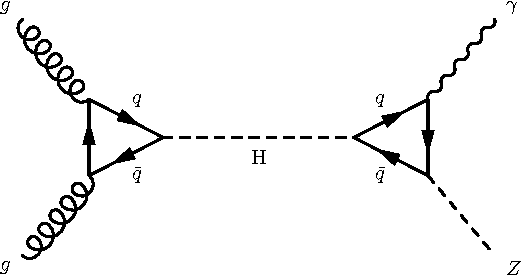
\includegraphics[width=\textwidth]{../dia/17.pdf}
    \caption{$gg \rightarrow Z\gamma$}
    \label{fey:17}
  \end{subfigure}%
  ~
  \begin{subfigure}[b]{0.3\textwidth}
    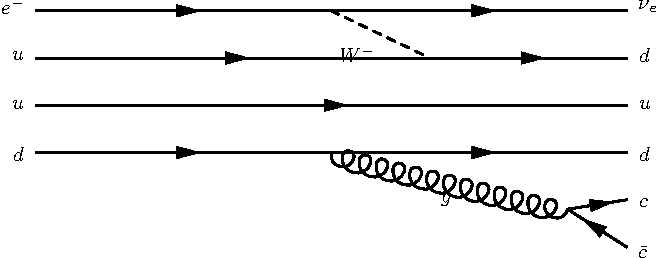
\includegraphics[width=\textwidth]{../dia/18.pdf}
    \caption{$gg\rightarrow t\bar{t}HH$}
    \label{fey:18}
  \end{subfigure}%
\end{figure}
\begin{figure}[h]
  \centering
  \begin{subfigure}[b]{0.3\textwidth}
    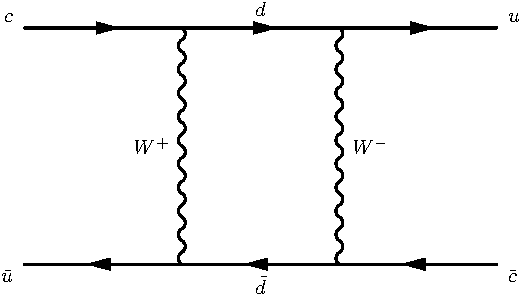
\includegraphics[width=\textwidth]{../dia/19.pdf}
    \caption{$D^0\longleftrightarrow \bar{D}^0$}
    \label{fey:19}
  \end{subfigure}
  ~
  \begin{subfigure}[b]{0.3\textwidth}
    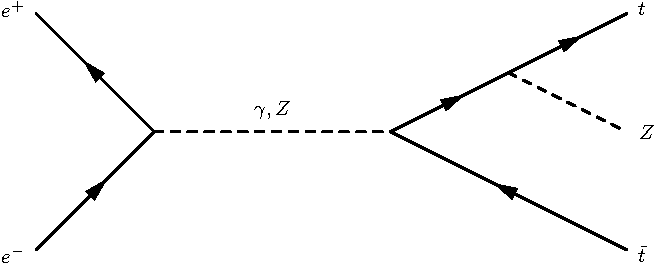
\includegraphics[width=\textwidth]{../dia/20.pdf}
    \caption{$e^+e^- \rightarrow t\bar{t}Z$}
    \label{fey:20}
  \end{subfigure}
\end{figure}
\restoregeometry
